%
% CHAPTER Versuch 4
%
\chapter{Pixelfehler}
Je nach Qualität des Bildsensors gibt es durch den Fertigungsprozess funktionsuntüchtige Pixel, welche das Bild verfälschen, diese gilt es in diesem Kapitel zu korrigieren.
\label{chap:Pixelfehler}

\section{Fragestellung, Messprinzip, Aufbau, Messmittel}
Um unser Testbild \ref{img:Grauwertkeil} zu korrigieren, gilt es nun den durch das Dunkelbild berechnete Offset der Pixel zu entfernen. Desweiteren wird das Bild noch durch das in V3 \ref{chap:VERSUCH_3} berechnete und normierte Weissbild geteilt um die Sensitivität anzupassen.
Im Anschluss wird uns ein Pythonskript TODO REF die differenz der einzelnen Bereiche zwischen dem Original Graukeilbild und dem korrigierten Graukeilbild berechnen. Hierzu wird das Bild zunächst in die einzelnen Graustufen zerlegt und im anschluss der durchschnittliche Farbwert dieser Graustufe wie auch die Standartabweichung, was dem rauschen der Pixel entspricht, berechnet. Durch vergleichen dieser Werte sollte sich eine Besserung des Bildes feststellen lassen. Die besserung sollte vorallem im beseitigen des rauschens liegen, was die Standartabweichung der einzelnen Keile sichtbar senken sollte.
\label{chap:VERSUCH_4_FRAGESTELLUNG}

\section{Messwerte}
\begin{figure}[H]
\centering
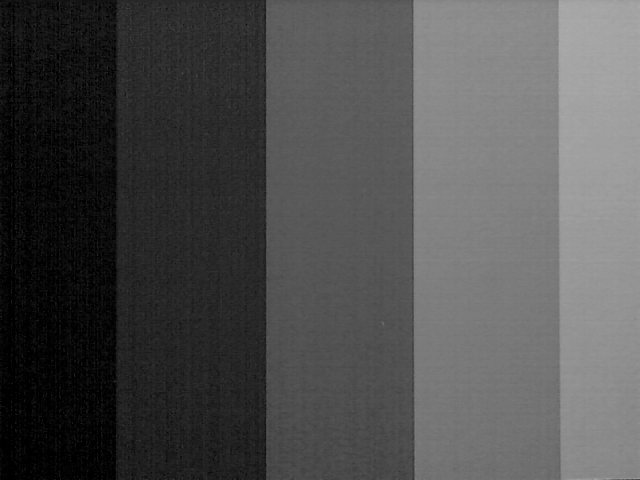
\includegraphics[width=150mm]{graustufen.png}
\caption{Markierter Offset}
\label{img:struckpixel.png}
\end{figure}
\label{chap:VERSUCH_4_MESSWERTE}

\section{Auswertung und Interpretation}
Bei genauerer Betrachtung des Kontrast maximierten Dunkelbildes \ref{img:struckpixel.png} fallen einige weisse Punkte ins Auge. Hierbei handelt es sich um hotpixel, welche durch längere Belichtungszeit in die Sättigung gehen oder um stuckpixel, welche sich stehts auf ihrem maximalwert bleiben $(rot markiert)$.
Ein Deadpixel ist ein pixel, welcher wie der Name bereits vermuten lässt nicht reagiert,somit ein pixel, welcher stets den wert 0 liefert, eine 0 wird als schwarz interpretiert. Ein schwarzer Pixel ist im Weissbild ziemlich auffällig, aber in unserem Fall nicht vorhanden. Die hier gefundenen schwarzen punkte sind lediglich durch Kontrast maximierung schwarz und somit keine deadpixel.
Zum korrigieren unseres Graukeilbildes wird zuerst das Dunkelbild abgezogen und anschließend durch das Weissbild dividiert. Die Formel $y = a\cdot x+b$ erklärt dieses Vorgehen. $y$ ist der durch die Kamera gelieferte Pixel. Dieser berechnet sich aus dem tatsächlichen Wert $x$ und der Sättigung $a$ zusätzlich beeinflusst noch der Offset $b$ das Ergebnis. Durch subtraktion des Offsets $b$ welcher uns das Schwarzbild liefert und anschließender division der Sättigung $a$ welche uns das Weissbild liefert erhalten wir die Formel: $x = \frac{y-b}{a}$ und somit den tatsächlichen Pixelwert.
Das im Pythonskript TODO REF berechnete neue Graustufenbild wird genau wie das Original in seine Graustufen zerlegt. Für diese Graustufen $(g1 - g5)$ werden jetzt jeweils Mittelwert und Standartabweichung berechnet TODO REF TABELLE. Hierbei wird deutlich, dass durch die Korrektur eine deutliche verbesserung erzielt wurde TODO REF TABELLE2, das Rauschen, sichtbar an der Standartabweichung, wurde um bis zu 79 \% verbessert.
In folgender Tabelle sind die Graustufen von g1 (Weiss) bis g5 (Schwarz) aufgelistet.

\begin{table}[H]
\centering
\begin{tabular}{l|ccccc}
Graustufe & Durchschnitt vorher & nachher & Stdabw vorher & nachher & Verbesserung in \% \\
\hline
g1 & 9.3699 & 9.2598 & 7.4903 & 7.1983 & 3.8981\\
g2 & 39.1486 &  38.6003 & 5.9921 & 4.5087 & 24.7560\\
g3 & 85.7785 & 83.8205& 6.9256 & 2.5537 & 63.1272\\
g4 & 126.9901 & 127.3212 & 8.8584 & 2.3224 & 73.7836\\
g5 & 152.3874 & 157.0740 & 9.1518 & 1.8588 & 79.6893\\

\end{tabular}
\end{table}
Bei genauerer betrachtung des Graukeilbildes fällt in der unteren rechten Ecke ein Fehler auf, welcher bei der aufnahme des Bildes gemacht wurde. Der Graustufenkeil lag nicht so, dass er da gesamte Bild ausfüllte, was jetzt als kleines dunkles Dreieck erkennbar ist. Damit dieser Fehler keinen Einfluss auf dem Durchschnittswert der weissen Graustufe nimmt, werden die untersten 20 Pixel ausgelassen, dies wird im Pythonskript \ref{lst:Graustufen} ersichtlich.
Die werte der Tabelle, worallem die letzte Spalte zeigen uns, dass unser Aufwand in den vorhergehenden Teilaufgaben nicht vergebens war, das rauschen wurde vorallem in den letzten drei Zeilen sehr effektiv beseitigt.
\label{chap:VERSUCH_4_AUSWERTUNG}